\subsection{Analyse}
\begin{figure}[H]
	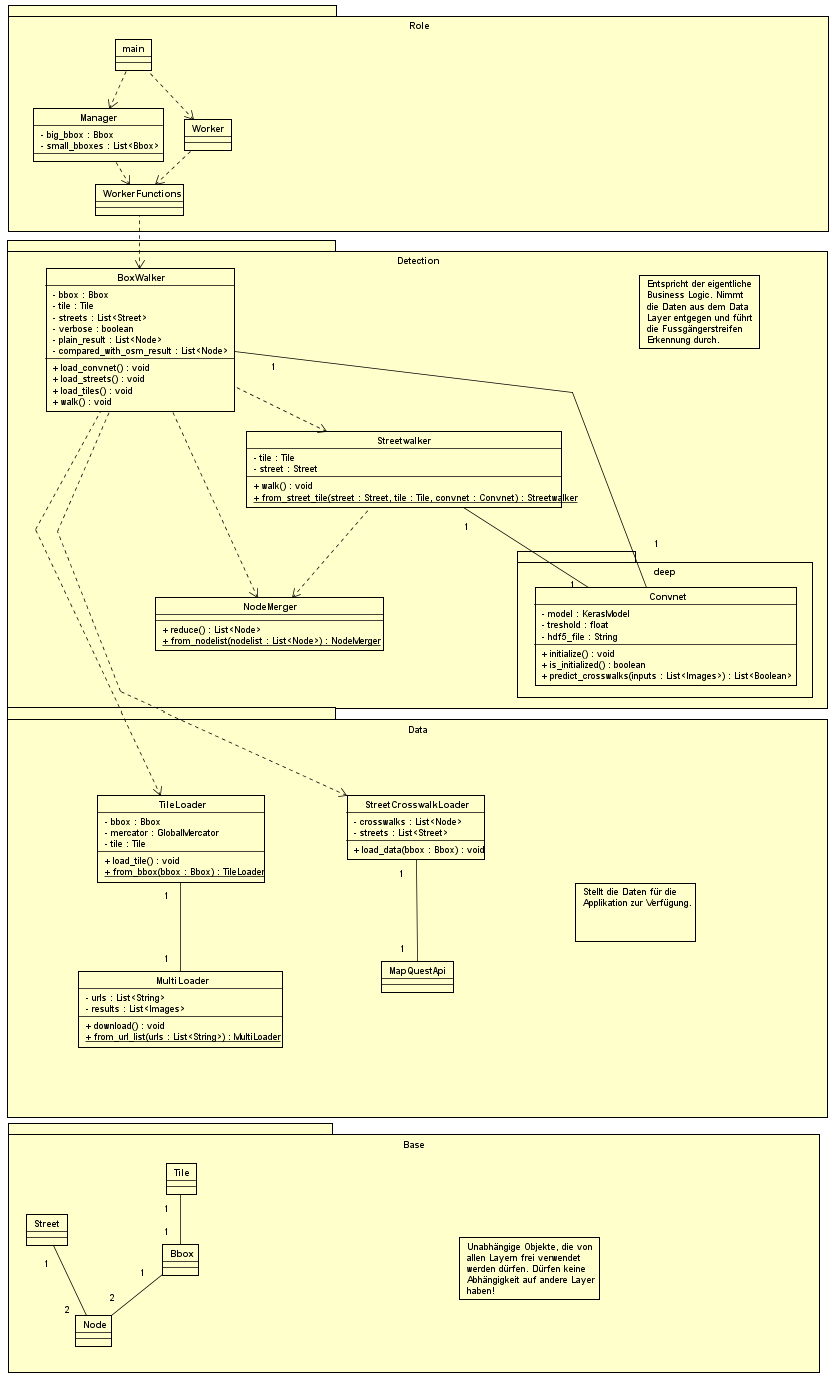
\includegraphics[width=\textwidth]{images/domain_model_komplett.png}
	\caption{Domain Modell}
\end{figure}
\subsubsection{Beschreibung Domain Modell}
Das Domain Modell besteht aus 4 Layern welche von oben nach unten auf einander aufbauen. Die Packages im Projekt sind gleich benannt wie die Layer. Die genauen Funktionen der entsprechenden Klassen sind im Kapitel Implementation einzusehen.
\begin{enumerate}
	\item Role - Parallelisierung
	\item Detection - Bilderkennung
	\item Data - Dataprovider
	\item Base - Grundelemente
\end{enumerate}

\subsubsection{Base}
Der Base Layer stellt Grundklassen wie ein Node oder eine Street zur Verfügung. Dieser Layer weisst nur Abhängigkeiten zu verwendeten Bibliotheken auf.

\subsubsection{Data}
Der Data Layer stellt den klassichen Data Link Layer dar. Er stellt Klassen zur Verfügung, um auf die entsprechenden Daten zuzugreifen. In unserem Fall sind es Orthofotos und Open Street Map Daten. Dieses Package benutzt den Base Layer.

\subsubsection{Detection}
Der Detection Layer beinhaltet die Funktionen zur eigentliche Bilderkennung. Dieser Layer holt seine Daten aus dem Data Layer und benutzt den Base Layer.

\subsubsection{Role}
Der Role Layer managt die Parallelisierung. Er greift ausschliesslich auf den Detection und auf den Base Layer zu.

Die Main Datei ist hier speziell zu erwähnen. Main verwaltet die Kommandozeilenaufrufe und startet das Programm dementsprechend. Diese Datei sollte eigentlich in einem eigenen Presentation Layer sein. Da wir jedoch keinen separaten Layer nur für eine Klasse machen, haben wir Main in den Role Layer verschoben.
